\newcommand{\lin}{linearne funkcije}

Linearna funkcija je polinomna funkcija prvog ili nultog stupnja.
Najčešće ju srećemo u sljedećem obliku:
\[f(x) = ax + b\]
\(x\) je argument funkcije, \(a\) zovemo linearni koeficjient, a \(b\) slobodni koeficjient.
Derivacija linearne funkcija ista je u svim točkama.
\begin{equation*}
    \begin{split}
        f'(x)   & = \lim_{\Delta x\to\infty} \frac{f(x + \Delta x) - f(x)}{\Delta x} \\
                & = \lim_{\Delta x\to\infty} \frac{f(a(x + \Delta x) + b) - f(ax + b)}{\Delta x} \\
                & = \lim_{\Delta x\to\infty} \frac{a\Delta x}{\Delta x} \\
        f'(x)   & = a
    \end{split}
\end{equation*}

\subsubsection{Domena i kodomena \lin}
    Domena i kodomena linearne funkcije su skup $\mathbb{R}$.
    \[f \colon \mathbb{R} \to \mathbb{R}\]

\subsubsection{Graf \lin}
    Graf linearne funkcije je pravac. Jednadžbu pravca nalazimo u implicitnom:
    \[Ax + By + C = 0,\]
    eksplicitnom:
    \[y = ax + b\]
    i segmentnom obliku:
    \[\frac{x}{m} + \frac{y}{n} = 1.\]
    Pravac se može opisati bili kojim od ovih oblika.
    Ako pogeldamo eksplicitni oblik pravca vidimo da osim o argumentu funkcije \(x\), graf ovisi i o koeficjientima \(a\) i \(b\).
    Mijenjajući \(a\) mjenjamo nagib grafa funkcije, a mijenjajući \(b\) mjenjamo odsjek na y-osi.

\subsubsection{Nultočke i točke u kojima graf sječe y-os \lin}
    Nultočke linearne funkcije možemo dobiti sljedećim izraom:
    \[f(x) = ax + b = 0\]
    Iz toga sljedi da linearna funkcija poprima vrijdnost 0 za:
    \[x = -\frac{b}{a}\]
    Vidimo da je nultočka jednistvena. (proizlazi iz tvrdnje u \ref{nultočke}.)
    
\subsubsection{Parnost i neparnost \lin}
    Linearna funkcija je parna za \(a = 0\):
    \begin{equation*}
        \begin{split}
            f(x) & = f(-x) \\
            ax + b & = -ax + b \\
            a & = 0
        \end{split}
    \end{equation*}
    \begin{figure}[ht]
        \centering
        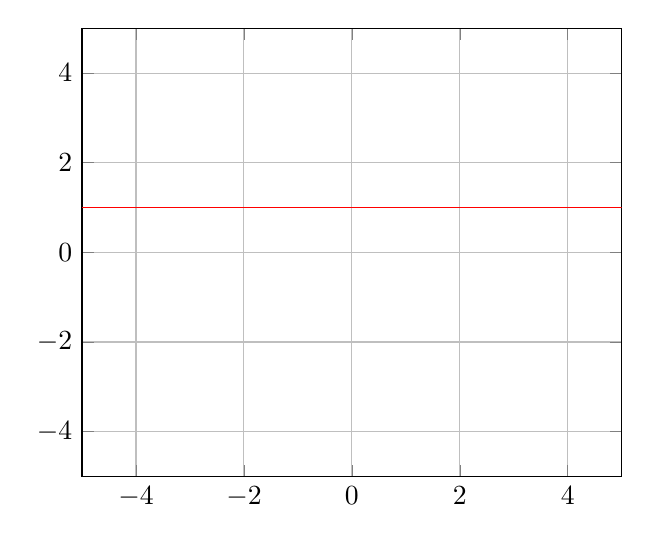
\begin{tikzpicture}
            \begin{axis}[
                grid=major,
                ymin=-5,
                ymax=5,
                xmin=-5,
                xmax=5,
            ]
                \addplot[
                    color = red,
                    samples = 100
                ]{1};
            \end{axis}
        \end{tikzpicture}
        \caption{Graf funkcije \(f(x) = 0 \cdot x + 1\)} 
        \label{fig:template}
    \end{figure}
    \\
    Linearna funkcija je neparna za \(b = 0\):
    \begin{equation*}
        \begin{split}
            -f(x) & = f(-x) \\
            -ax - b & = -ax + b \\
            b & = 0
        \end{split}
    \end{equation*}
    \begin{figure}[ht]
        \centering
        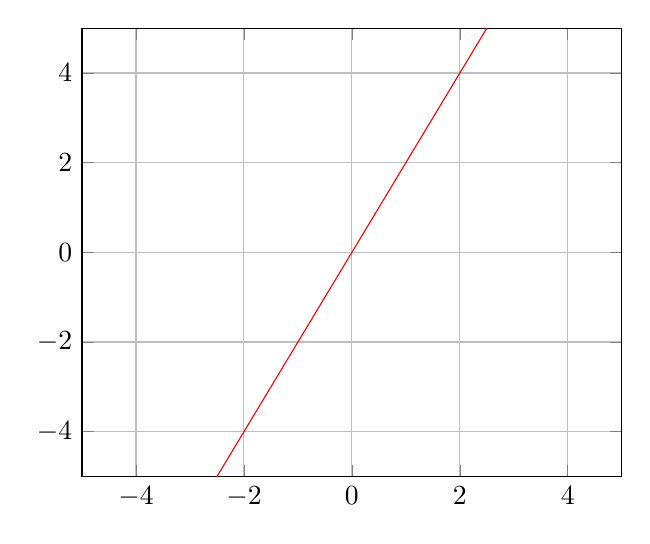
\begin{tikzpicture}
            \begin{axis}[
                grid=major,
                ymin=-5,
                ymax=5,
                xmin=-5,
                xmax=5,
            ]
                \addplot[
                    color = red,
                    samples = 100
                ]{2 * x};
            \end{axis}
        \end{tikzpicture}
        \caption{Graf funkcije \(f(x) = 2 \cdot x + 0\)} 
        \label{fig:template}
    \end{figure}
    \\

\subsubsection{Periodičnost \lin}
    Linearna funkcija je periodična za sve periode \(P\), \(P \neq 0\) samo kada je \(a = 0\).
    \begin{equation*}
        \begin{split}
            f(x + P)        & = f(x) \\
            a(x + P) + b    & = ax + b \\
            0 \cdot (x + P) + b & = 0 \cdot x + b \\
            b               & = b
        \end{split}
    \end{equation*}

\subsubsection{Monotonost \lin}
    Linearna funkcija je strogo rastuća, strogo padajuća ili konstantna ovisno o nagibu \(a\). 
    Konstantna funkcija je rastuća i padajuća jer zadovoljava uvjete navedene u \ref{mono}.
    \begin{figure}[ht]
        \centering
        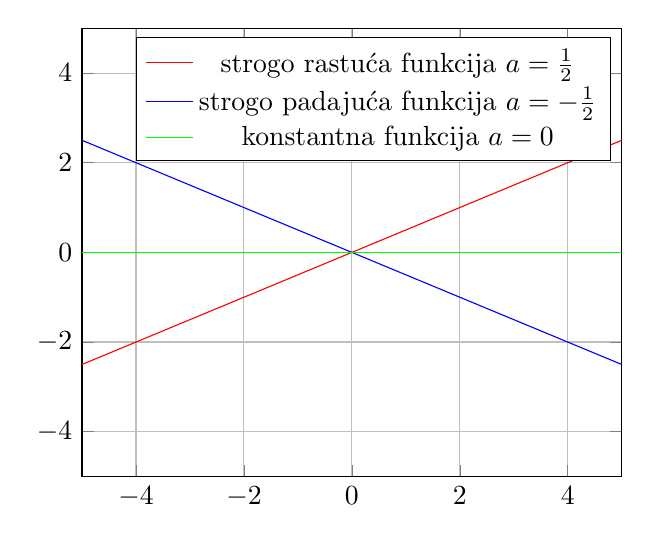
\begin{tikzpicture}
            \begin{axis}[
                grid=major,
                ymin=-5,
                ymax=5,
                xmin=-5,
                xmax=5,
            ]
                \addplot[
                    color = red,
                    samples = 100
                ]{1/2 * x};
                \addlegendentry{strogo rastuća funkcija \(a = \frac{1}{2}\)}
                \addplot[
                    color = blue,
                    samples = 100
                ]{-1/2 * x};
                \addlegendentry{strogo padajuća funkcija \(a = -\frac{1}{2}\)}
                \addplot[
                    color = green,
                    samples = 100
                ]{0};
                \addlegendentry{konstantna funkcija \(a = 0\)}
            \end{axis}
        \end{tikzpicture}
        \caption{Primjer monotonosti linearnih funkcija} 
        \label{fig:template}
    \end{figure}
    \\

\subsubsection{Omeđenost \lin}
    Linearna funkcija je omeđena samo kad je konstantna.
    \[m = M = f(x)\]

\subsubsection{Injektivnost i surjektivnost \lin}
    Linearna funkcija je bijekcija za \(a \neq 0\). Injekcija je jer vrijedi:
    \begin{equation*}
        \begin{split}
            f(x_1)      &= f(x_2) \\
            ax_1 + b    &= ax_2 + b \\
            x_1         &= x_2
        \end{split}
    \end{equation*}
    Surjekcija je jer vrijedi:
    \[\forall y \in K_f, \exists x \in D_f, y = f(x),\]
    a domena i kodomena linearna je skup $\mathbb{R}$.
    Bijekcija je jer je injekcija i surjekcija.
    Ako je \(a = 0\) funkcija je surjekcija, vrijedi izraz gore.
    
\subsubsection{Inverz \lin}
    Inverzna funkcija linearnoj je također linearna funkcija:
    \[f^{-1}(x) = \frac{x - b}{a}\]
    \begin{figure}[ht]
        \centering
        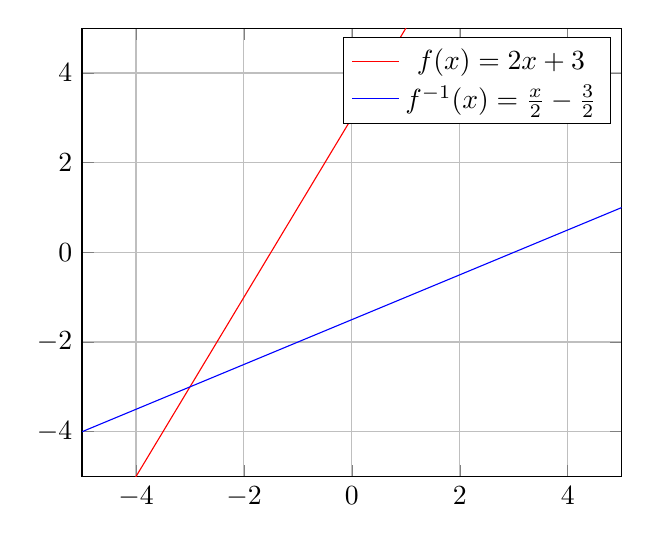
\begin{tikzpicture}
            \begin{axis}[
                grid=major,
                ymin=-5,
                ymax=5,
                xmin=-5,
                xmax=5,
            ]
                \addplot[
                    color = red,
                    samples = 100
                ]{2 * x + 3};
                \addlegendentry{\(f(x) = 2x + 3\)}
                \addplot[
                    color = blue,
                    samples = 100
                ]{x / 2 - 3 / 2};
                \addlegendentry{\(f^{-1}(x) = \frac{x}{2} - \frac{3}{2}\)}
            \end{axis}
        \end{tikzpicture}
        \caption{Grafovi funkcije i njenzinog inverzna} 
        \label{fig:template}
    \end{figure}
    \\